\chapter{Photon Detector}
\label{ch:photon}
\section{Introduction}

Liquid argon is an excellent scintillating medium. With an average
energy needed to produce a photon of 19.5~eV (at zero field) a typical
particle depositing 1~MeV in liquid argon will generate 40,000~photons
with wavelength of 128~nm. At higher fields this will be reduced but
at 500~V/cm the yield is still about $\sim$20,000~photons per
MeV. Roughly 1/3 of the photons are promptly emitted after about 6~ns
while the rest are are emitted with a delay of 1100-1600~ns. LAr
is highly transparent to the 128~VUV photons with a Rayleigh
scattering length and absorption length of 95~cm and >200~cm
respectively. The relatively large light yield makes the scintillation
process an excellent candidate for determination of $t_{0}$ for
non-beam related events. Detection of the scintillation light may also
be helpful in background rejection.

\section{Requirements and Goals}

\subsection{Beam-based physics}

There are no requirements for the beam-based physics program, as the
machine clock will provide a $t_{0}$ with roughly 10 $\mu$s
resolution. Given that the electron drift is 1.6 mm/$\mu$s the
uncertainty to the electron lifetime correction is small is the beam
timing is used. The photon system can be useful in determining the
$t_{0}$ of cosmic ray events and events from radiological decays as
well as giving a handle to the location of beam events in the LAr
volume wuth respect to fiducial boundaries. The impact of the LAr
scintillaiton light on the detector performance needs to be
determined, but it is not expected that the reduction in backgrounds
for the oscillation program will introduce additional requirements to
the photon system design.

\subsection{Proton decay and atmospheric physics}

The photon detector system must provide the t$_0$ for non-beam related
physics channels if a correction for electron recombination during
drift is to be applied. The requirements for electronics and hadronic
energy resolution for the proton decay and the atmospheric neutrino
program are $1\% / \sqrt{E(GeV)} \bigoplus 1\%$ and $30\% /
\sqrt{E(GeV)}$ respectively. With these resolutions the collected
charge must be accurately corrected for recombination. Therefore the
photon system must provide a $t_{0}$ for particles with >100 MeV with
>95\% efficiency in the fiducial volume of the detector.

\subsection{Low-energy physics}

Supernova events will produce neutrinos down to about
$\sim$5~MeV. Studies have estimated the momentum resolution for 5 MeV
electrons to be 20\% using only TPC information and assuming a highly
efficient trigger and an electron lifetime of 5 ms. The impact of
various detector resolutions on the physics potential of LBNE has not
been studied in detail. At present there is no strong requirement that
the energy resolution must be better than 20\% so no requirement on
the photon system trigger efficiency is set at this time. However it
is clear that if a detector design can be found the energy resolution
would greatly improve. A goal of the photon detection R\&D is to
develop a system with the lowest possible threshold for a reasonable
cost. At time of the start of final design a final decision as to the
configuration will need to be made based on cost and added physics
capability.

\subsection{Required Performance}

To achieve the physics goals in the previous section the performance
of the photon detection system must be understood. The prototype
readout electronics described in section~\ref{sec_elec} have been
shown to detect the single p.e. signals associated with the late
scintillation light but future versions may sacrifice this ability to
mitigate high channel costs. It is assumed that the physics goals of
the photon detection system will be met using on the prompt
scintillation light.

The performance, or overall photon collection efficiency, is given by
the following, where it is assumed only prompt light is collected:

\begin{equation}\label{eff_eqn}
\frac{N_{pe}}{MeV} = N_{128}\cdot \epsilon_{geom} \cdot \epsilon_{E} \cdot
\epsilon_{mesh} \cdot \epsilon_{conv} \cdot \epsilon_{capt}
\epsilon_{tran} \cdot \epsilon_{QE} 
\end{equation}

The efficiencies leading to the overall number of photo-electrons
collected by the photon detection system, $\frac{N_{pe}}{MeV}$, are given
in table~\ref{Table-Eff}.


\begin{cdrtable}[Individual photon collection efficiencies]{clcl}{example}
{Individual photon collection efficiencies}
 Factor & Description & Value & Comments \\ \toprowrule
   $\epsilon_{geom}$ & geometric acceptance & 0.0036 & historical
      average  \\ \colhline
      $\epsilon_{E}$ & field correction & 0.6 & 500~V/cm  \\ \colhline
      $\epsilon_{mesh}$ & TPC wire shadowing & .83 (30-150$^{\circ}$)
      & falls off sharply~\cite{HimmelMesh}  \\ \colhline
      $\epsilon_{conv}$ & TPB conversion & 1 & see
      ref.~\cite{bib:gehman}  \\ \colhline
      $\epsilon_{capt}$ & waveguide incident & 0.5 & about half
      converted photons\\ \colhline
      &  & & travel into waveguide  \\ \colhline
      $\epsilon_{tran}$ & waveguide transmission & TBD  & prototype
      dependent  \\ \colhline
     $\epsilon_{QE}$ & SiPM QE & .31  & SensL b-series  \\
\end{cdrtable}


Using equation~\ref{eff_eqn} it is seen that to detect a
2~p.e. signal, likely to be discriminated from noise, the transport
efficiency of 1.2\%. Of course this value is very position dependent
as the geometric acceptance, wire shadowing, and transport corrections
all depend on the location of the event. Figure~\ref{fig:photon_map}
shows the probability of (?) MeV energy deposition neing detected in
the photon detectors. 

\begin{cdrfigure}[Probability of photon being detected in
  detectors when depositing energy]{photon_map}{Photon map giving the probability of photon being 
  detected in the photon detectors when depositing energy at map location. \fixme{(need
  general TPC cell map with better description)}}
  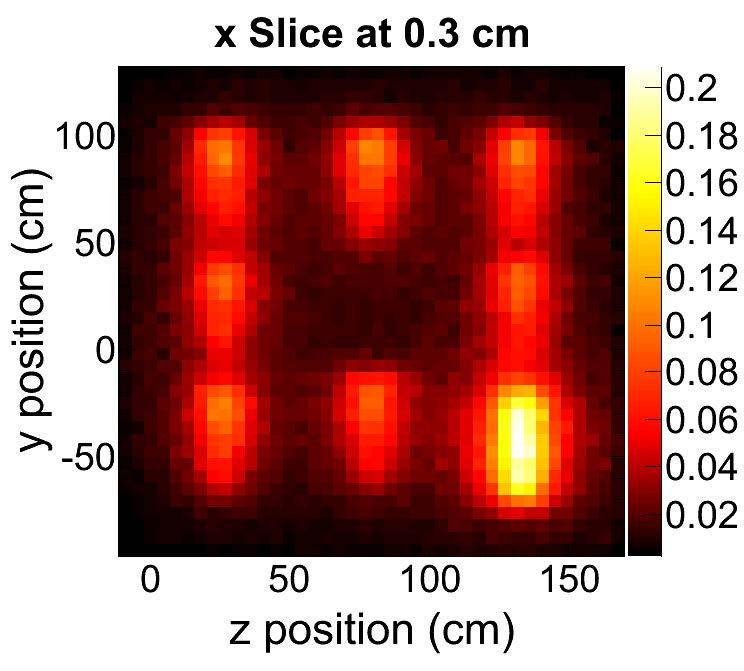
\includegraphics[width=0.4\textwidth]{35t_map.jpg}
\end{cdrfigure}


The TPC wire mesh shadowing is also quite location dependent as photon
angles, relative to the wire plane, lead to rapid loss in transmission
below 30$^{\circ}$ and greater than 150$^{\circ}$. Lastly the photon
detector paddles themselves can have position dependent response to
incident photons due to the attenuation length of the waveguide. The
photon detector simulation, which is nearing stable operation, will be
able to better estimate the efficiencies coming from geometric
acceptance correction.

\subsection{General Considerations}

In the event that higher photon collection efficiencies can be
achieved it should be possible to improve the energy resolution of the
detector by adding the photon yield to the electron yield information.
However this requires several orders of improvement in light
collection efficiency so it is beyond the scope of present designed.

\section{Photon Detector Prototype Designs}

All design considered for the photon detector have been based on the
use of wavelength-shifting coating, or bulk doping, of plastic
materials coupled to silicon photomultipliers (SiPMs). The reference
design~\ref{sec_bars} utilizes a coated acrylic waveguide coupled to
SiPMs. Alternatate designs, desribed in the following section, have
been developed to optimize coverage, cost, and attenuation length. 

\subsection{Cast or Bulk doped acrylic bars}
\label{sec_bars}

The reference design for the photon detection system is based on light
guides that are coated with wavelength shifter. The 128 nm
scintillation photons from liquid argon interact with the wavelength
shifter on the light guide surface and 430 nm light is re-emitted in
the bar.  The light guide channels the light to photodectors at its
end.

A schematic drawing of a light guide with its photosensors is shown in
Figure~\ref{fig:WaveguideSketch}. The prototype light guides are bars
with a footprint 2.54 cm $\times$ 0.6 cm.  The concept is described in
Ref.~\cite{bib:MITbars}.

\begin{cdrfigure}[Schematic drawing of a light guide with its
      photosensors]{WaveguideSketch}{Schematic drawing of a light guide with its
      photosensors. The bars have embedded wavelength shifter (WLS),
      either TPB or bis-MSB. Three SiPMs collect the waveshifted
      photons that have been internally reflected to the bar's end. \fixme{Fuzzy at this size}}
    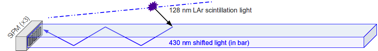
\includegraphics[width=.85\columnwidth]{cast-acryl-lightguide}
\end{cdrfigure}

The wavelength shifter converts VUV scintillation photons striking it
to 430~nm photons inside the bar, with an efficiency of $\sim$50\% of
converting a VUV to an optical photon~\cite{bib:gehman}.  A fraction
of the waveshifted optical photons are internally reflected to the
bar's end where they are detected by SiPMs whose QE is well matched to
the 430~nm waveshifted photons. The light guides were made with one of
two wavelength shifters: the conventional TPB
(1,1,4,4-tetraphenyl-1,3-butadiene) and the less expensive alternative
bis-MSB (1,4-bis-(o-methyl-styryl)-benzene). Preliminary studies with
a VUV monochromator show that the two wavelength shifters compare
favorably in their waveshifting efficiency~\cite{bib:baptistaJINST}. A
testing program is currently underway to compare their relative
performance in liquid argon.

The prototype light guides being studied at Indiana are made with
different three technologies. These technologies are listed in
Table~\ref{tab:lightGuides}.

\begin{cdrtable}[Light guide technologies]{ c l  l }{lightGuides}
{Light guide technologies}
  Label & Light Guide Technologies \\ \toprowrule
  (a) & clear acrylic, dip-coated   \\ \colhline
      (b) & doped Eljen PVT light guide, dip-coated   \\ \colhline
      (c) & doped Eljen polystyrene light guide, dip-coated    \\ 
\end{cdrtable}



(a) The clear acrylic bars are made from blanks of commercially
available Lucite-UTRAN cast UVT acrylic sheet that has been laser-cut
and diamond-polished into bars of the proper size.  Lucite-UTRAN has
the longest attenuation length of the acrylics
tested~\cite{bib:mufsonJINST}.  The
Eljen\footnote{http://www.eljentechnology.com} bars are commercial
light guides that are doped with J2 green fluor (equivalent to Y11).
Two types of light guides were purchased from Eljen.  (b) The light
guides were fabricated from polyvinyl toluene (PVT).  These are the
standard Eljen product EJ-280.  The quantum efficiency of the
fluorescent dopant in EJ-280 is 0.86, so the second shift in
wavelength does not markedly degrade the photon detector efficiency.
(c) The light guides were fabricated from polystyrene.  These light
guides were ordered because PVT bars can craze if cooled too rapidly.
Although the PVT light guides may be brighter, no instance of crazing
has ever been observed in polystyrene light guides.

For the acrylic light guides, the WLS must be embedded in the plastic
at the bar's surface so that 128~nm scintillation photons can generate
optical 430~nm photons within the volume of the plastic.  Otherwise
the VUV photons will not be trapped by the light guide.  For the Eljen
bars, the wavlength shifter can either be embedded in the plastic as
with the acrylic.  Or it can be deposited on a plate or film placed in
proximity to the light guides.  The J2 wavelength shifter then
converts the resulting 430~nm photons inside the light guides where
they are channeled to the photodetectors.

To embed the WLS at the surface of the light guides, a ``dip-coating''
process was developed at Indiana University.  Before the WLS was
applied to the acrylic bars, they were annealed at 80$^\circ$C for one
hour.  The Eljen bars were not annealed.  The WLS was dissolved in the
organic solvent dichlormethane (CH$_2$Cl$_2$).  For these waveguides
there were 5 gm of wavelength shifter dissolved in 1,000~gm of DCM.  A
series of experiments showed that this concentration was optimum.  A
bar was first dipped into the WLS mixture for 15 seconds and then
removed.  It was then hung in the dark for at least two hours to dry.
Once dry, the ends of the bars were flycut.  Currently designs are
being fabricated that put an acrylic plate painted with WLS or a thin
film impregnated with WLS in front of the Eljen light guides .

In summer 2015 these designs will all be tested side-by-side at the
TallBo dewar facility at Fermilab under uniform, low-contamination
conditions.  In addition to the designs described above, these tests
will include photon detector designs from Colorado State University
and Louisiana State University.  This experiment will compare the
relative performance and the absolute efficiency for all designs
scaled to 1.5 m.

\subsection{Fiber-embedded bulk acrylic plate}

At LSU, Thomas Kutter and team have developed a VUV photon detector
design for a large LAr detector that overcomes some of the
shortcomings of the present LBNE baseline photon detectors. The LSU
photon detector design allows for a very large area coverage thereby
increasing the geometrical acceptance of the photon detectors. The
number of required SiPMs and readout channels per unit detector area
covered with photon detection panels has been significantly reduced to
keep the overall cost for the photon detection system at or below the
present design while increasing the geometrical acceptance at the same
time.

The photon detection system consists of a TPB coated acrylic panel
with an embedded S-shaped wavelength shifting (WLS) fiber. The fiber
is read out by two SiPMs, which are coupled to either end of the fiber
and serves to transport the light over long distances with minimal
attenuation. The double-ended fiber readout has the added benefit to
provide some position dependence to the light generation along the
panel by comparing relative signal sizes and arrival times in the two
SiPMs. Figure \ref{fig:1-LSU} show a drawing of the layout and a
picture of a prototype photon detection panel in the test stand at
LSU.  The incoming 128nm VUV Ar scintillation light will be converted
by the thin TPB layer on the acrylic panel and re-emitted with
wavelength peaking at 430nm in an isotropic way. About 50\% of the
light would be emitted into the acrylic panel where some fraction will
be absorbed by the WLS fiber and converted to light with a peak
intensity of about 480 - 500~nm. The green light exiting the fiber is
well matched to the peak photon detection efficiency of typical SiPMs.

\begin{cdrfigure}[LSU photon-detection panel]{1-LSU}{LSU photon-detection panel. Technical drawing of a $20"\times4.33"$ acrylic panel with embedded WLS fiber (left) and picture of a prototype in test set-up at LSU (right) with the same dimensions.}
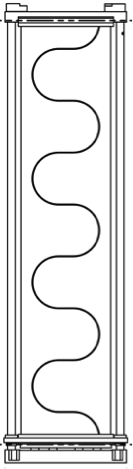
\includegraphics[width=0.25\linewidth]{LSU_panel_drawing.png}
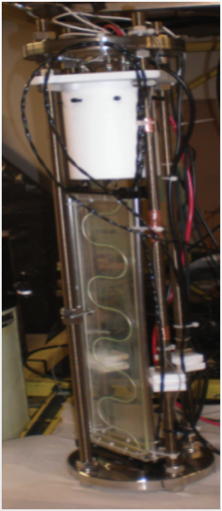
\includegraphics[width=0.45\linewidth]{LSU_panel_prototype.png}
\end{cdrfigure}



\subsection{LSU Photon detection panel production}
The photon detection panels are produced from 0.25\" thick
sheet UVT acrylic and cut to size. For a first series of prototypes
the acrylic panel dimensions were chosen to closely match the area of
4 bars of the LBNE baseline photon detection system.  The groove is
cut with a CNC mill in several passes to achieve good groove surface
quality, which is important for good light transmission from the bulk
acrylic to the fiber. The panels are dip coated with TPB and left to
dry prior to insertion of the WLS fiber. Panels with two and three
layers of fibers inserted and glued into the groove have been
produced. Fiber ends are cut and polished.  The resulting acrylic
panels are then inserted into a custom made mechanical frame which was
designed by David Warner at CSU. The end caps of the mechanical frame
house one SiPM on either end. The presently used 6x6 mm2 active area
SiPM are spring mounted to ensure good contact between the active area
and the fiber ends.  The leads of the SiPMs are connected to a small
PCB onto which ~2m long twisted pair coax cables are soldered to
supply the SiPM with a bias voltage and read out signals. The other
cable ends are typically connected to pre-amplifiers before leading to
a DAQ system.  Components for the photon detection panels are
inspected at all stages of the manufacturing process for quality. Due
to the small number of panels produced to date no quantitative quality
control parameters have been defined yet.  Proper connectivity of the
fully assembled units are tested in a setup at LSU using a LED
flasher. If LED light signals are seen the panel is successively
immersed in gaseous argon (GAr) along with an alpha source. The
observation of argon scintillation light originating from alpha
particles and cosmic-rays penetrating the GAr volume allows for a
relatively quick quality control check of a completed photon detector
at room temperature.

\subsection{Proof of concept and prototype detector results}
Several photon detector panels of $20" \times 4.33"$ have been
produced and two have been tested in a LAr test stand at CSU. The
detectors submitted to the cold test have 3 and 2 embedded fibers,
respectively, but are otherwise produced in the same way. The data
taking in LAr included self triggered alpha source scans as well as
cosmic runs with a muon hodoscope providing a trigger for near
vertical muons penetrating the LAr volume.
\paragraph{Alpha source runs:} The alpha source was placed at a distance of about 1" in front of the center line of the photon panel and moved to 20 different positions spaced about 1" apart from neighboring positions. At each position 5000 signal traces were recorded and measurements were repeated for three of the positions to check the reproducibility of the measured light yield. Figure \ref{fig:2-LSU} shows results for both successively measured panels. The red and blue dots show the mean light yield values in units of p.e. (photo electron equivalents = no. of fired SiPM pixels) for the SiPM on the top and bottom end of the panel as function of source position. Green dots show the sum of both channels. The summed signals provide a very uniform detector response for the entire panel and independent of the alpha source position. The data also indicate good reproducibility for the doubly measured positions.
The 3-fiber panel shows about 50\% more light when compared to the
2-fiber panel which is in good agreement with expectations. It needs
to be pointed out that the LAr purity was not monitored and that
measurements for the two panels were performed sequentially after
refilling the dewar with LAr. However, the liquid argon for both
measurements came from the same batch which motivates the assumption
that the purity for both measurements was very similar.

%
\begin{cdrfigure}[Light yield for the fiber LSU PD panels with alpha source in
  LAr]{2-LSU}{Light yield for the 3 (left) and 2 (right) fiber LSU photon
  detection panels in response to a 1" distant alpha source in
  LAr. Red and blue symbols represent the mean light yield over 5000
  trigger events from a single SiPM each and green points represent
 the summed signal from both SiPMs.}
\resizebox{.48\textwidth}{!}{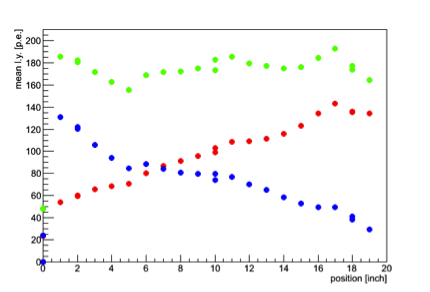
\includegraphics[width=0.45\linewidth]{LSU_panel_prototype1_ly-position.png}}
    \resizebox{.48\textwidth}{!}{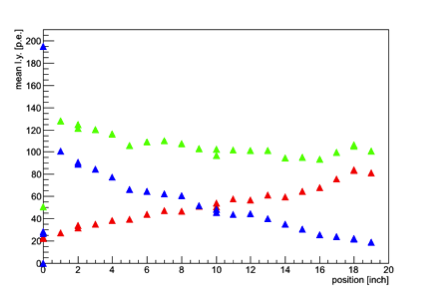
\includegraphics[width=0.8\linewidth]{LSU_panel_prototype2_ly-position.png}}
\end{cdrfigure}

%
\paragraph{Cosmic trigger runs:} Two $ 1" \times 10"$ wide scintillator counters were placed above and below the dewar to form a muon hodoscope and to select near vertical muons traversing the LAr volume. The 3-fiber LSU panel and one LBNL/Elgin Bis-MSB doped polystyrene bar of LBNE baseline dimensions and read out by three SiPMs were simultaneously inserted in the LAr. The setup allowed the study of the response of these photon detectors to scintillation light created by penetrating cosmic muons. A detailed quantitative comparison of the relative light yield was not possible with this setup due to large systematic uncertainties in the position dependence of the scintillation light generation by the triggering cosmic muons. A qualitative comparison of the detector responses, taken as the signal sum of 3 and 2 SiPMs for the Elgin bar and the LSU panel, respectively, shows comparable light yields as shown in figure \ref{fig:3-LSU}. 
        
%
%
\begin{cdrfigure}[Summed charge plots of SiPMs in response to muon hodoscope trigger]{3-LSU}{Scatter plot of the summed charge of 3 SiPMs coupled to the
 LBNL/Elgin Bis-MSB doped bar and the summed charge of 2 SiPMs for
 the 3-fiber LSU panel in response to an external muon hodoscope
 trigger. The right plot shows a zoomed version of the left plot.}
   \resizebox{.48\textwidth}{!}{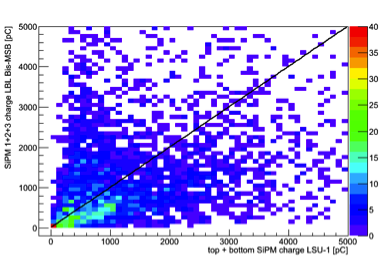
\includegraphics[width=0.45\linewidth]{LSU_panel_prototype_charge.png}}
   \resizebox{.48\textwidth}{!}{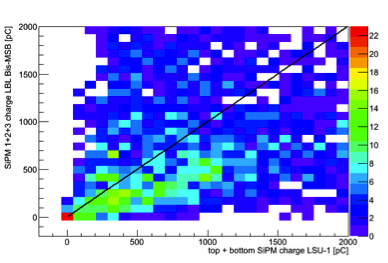
\includegraphics[width=0.8\linewidth]{LSU_panel_prototype_charge_zoom.png}}
\end{cdrfigure}

%

\subsection{R\&D Work in progress and present Plans }

After the construction and proof of principle test of the LSU style
photon detection panels we manufactured several 2.17m long and 110mm
(=4.33") wide panels to demonstrate the scalability of the design.  At
the time of writing tests in the large LAr dewar at CSU are in
progress.  We are performing alpha source scans and cosmic muon runs.
The alpha source scan runs are arranged such that the source
illuminates two photon detectors at the same time.  This setup
facilitates quantitative and relative light yield comparison between
different photon detector designs in the same LAr bath with a well
defined VUV light source.

Manufacturing and testing of wider panels is under consideration to
maximize the photon detector panel area in the ELBNF LAr far
detector. The goal is to cover the entire anode plane assembly (APA)
area with photon detectors embedded into the APA frame.  Another
important measurement goal is to establish the energy threshold of the
photon detection panels. A study will be conducted for the photon
detectors presently installed in the 35t detector using Michel
electrons. The 35t detector contains one of the 3-fiber LSU photon
detection panels. In addition, alpha source runs in a well-controlled
and monitored LAr setup may provide information on the particle energy
threshold for observation of VUV scintillation light.  The measurement
of a photon detector panel's light yield as function of the source
distance is another key measurement to estimate the response and
sensitivity of the full photon detection system in a LAr
detector. Results will be useful to validate MC simulations.  We are
exploring options to perform these tests in the large dewar setup at
CSU or alternatively in the TallBo setup at FNAL.

The TPB coating procedure of the acrylic panels has not yet been
optimized and improvements may be possible. We foresee a systematic
study to identify parameters in the TPB dip and alternatively the
evaporation coating procedure to maximize the light yield of resulting
samples. These tests will be performed on small
$10\times10~\mathrm{cm}^2$ acrylic panels with a U-shaped embedded WLS
fiber.  On the software and analysis side we are in the process of
improving our tools to study position dependence for alpha source run
data using relative signal timing and size. Furthermore, we plan to
continue work on analysis algorithms to identify the late light
component from argon scintillation.

Finally, early exploratory work on wallpapering the TPC cathode planes
with TPB coated Tetratex foils and observing the shifted light with
suitably installed photon sensors in combination with light collector
cones will be pursued and explored more rigorously to provide timely
results.


\subsection{Fiber bundle with WS-coated readiator}

The driving cost of the photon detector system is readout
electronics. A reduction in attenuation length has been observed for
acrylic waveguids that have been doped with TPB. Once scenario to
address this reduction is to populate the PD system with half-length
paddles. Of course this leads to an increase in the number of readout
channels. While it may be possible to combine readout channels to
mitigate the increase in overall number a more desirable soultion
would be to address the attenuaton length issue.   

To mitigate the reduced attenuation length of acrylic and polystyrene
that have been either doped with or coated with TPB the CSU group has
been developing an alternative design that is based on UV to blue
wavelength shifting fiber (Y11) that has not been treated with TPB.  A
thin TPB coated acrylic radiator located in front of a close packed
array of WLS fibers. Figure~\ref{fig:fiber_bundle} is a photograph of the
fiber-bundle prototype. 

\begin{cdrfigure}[Fiber-bundle PD prototype (early one-sided
  version)]{fiber_bundle}{Photograph of fiber-bundle PD prototype (early one-sided
  version). The thin TPB-coated radiator is mounted on top of the
  prototype in the image.}
  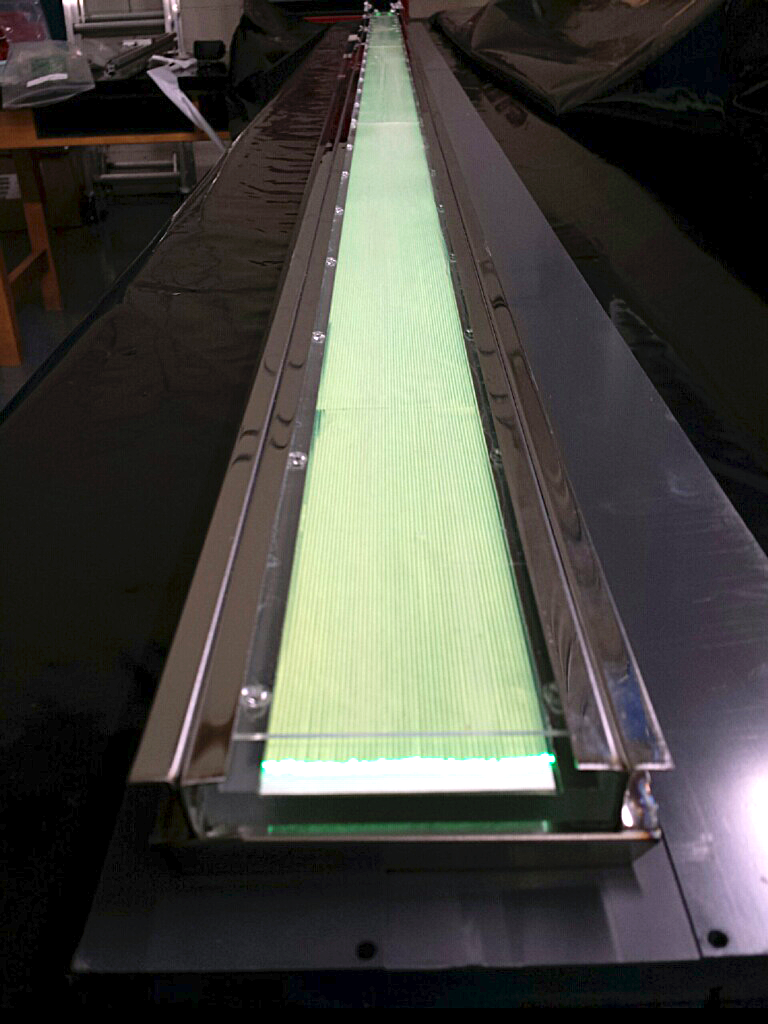
\includegraphics[width=.4\columnwidth]{fiber_bundle_1.png}
\end{cdrfigure}


The VUV photons are incident on the TPB-coated plastic radiator and
roughly half of the photons converted in the radiator are incident on
the bundle fiber bundle. The photons in the Y11 fiber are then which
are directed onto SiPMs at one end. The Y11 fiber (from Kuraray ) have
mean absorption and emission wavelengths of about 440 nm and 480 nm
respectively.  The attenuation length of the Y11 fibers is given to be
greater than 3.5 m at the mean emission wavelength, which allows
production of full-scale (2.2 m length) photon detector paddles.

First prototypes of this design utilized two rows of fibers with a
reflecter behind the doubled row to redirect the ~400~nm photons back
through the two rows if they weren't absorbed on the first pass
through. Based on data taken at the CSU Cryogenic Detector Development
Facility (CDDF) and the Fall 2014 FNAL Tallbo test, only a single row
design could be considered - and is currently under development. Data
taken at both tests showed that the front row of fibers collected
twice as much light as the back row of fibers. The current design
utilizes teo single rows of fibers back-to-back with layers of Tyvek
diffuse reflector in between.

Another benefit of this design is that an arragement with back-to-back
rows of fibers separated by an opaque relector arranged would then
face into different TPC cells allowing additional information to be
used in the disambiguation of the TPC signals coming from wire
wrapping on the APA frames. A further benefit of the design could be
compatibility with concepts where the walls of the detector are
covered with TPB coated material shifting the VUV photon to blue and
then the WS-fiber can capture the emitted light. Further study is
required to determine the effect of these enhancements on physics
reach of the detector. 

To fully exploit this approach several design optimizations need to be
be examined including the following:

\begin{itemize}

\item{TPB coating thickness on thin radiator}

\item{Double-ended readout. If the fibers are readout out from both
  ends and the corresponding channels are ganged onto one readout
  channel an increase in channel output can be obtained without
  significant cost.}

\item{Use of custom doped fibers to best match the QE response of the
  SiPMs and the emission sepctrum of the TPB.}

\item{Remove the radiator and coat the TPB directly onto the outer
  fiber cladding of the Y11 fibers. Since the fibers are double-clad
  it may be the case that the attenuation lenth of the fibers is not
  altered byt the TPB application. The geometry of the close-packed
  fiber row may lead to increased photon (400~nm) collection}

\end{itemize}

The cost of this design is comparable to that of the bar-based design
but is slightly more complex to fabricate - although the Y11 fibers
are commercially available which is an attractive feature. The
engineering aspects of the design will be discussed in the approariate
section of this chapter. 

\section{Silicon Photo-multipliers}

Silicon Photomultipliers (SiPMs) have been selected as photon
detectors for the far detector LArTPC photon detection system. SiPM is
a photo detection device sensitive to single photons with excellent
linearity range in collecting multiple photons.  SiPM consists of a
large avalanche photodiode (APD) array built on a common silicon
substrate. APDs operate in Geiger mode.

SiPMs have been developing at a very fast pace in recent years, in
response to the needs of medical industry. As a result, the price of
SiPMs has gone down, while their performance has greatly
improved. There are a number of characteristics that make SiPMs an
attractive choice as photo-detectors for the PD system.

\begin{itemize}

\item{High photon-detection efficiency (PDE) up to 40-50\% at the
  peak detection wavelength. }

\item{High intrinsic gain at ranging from 105 to 107 depending on the
  overvoltage.}
\item{Low dark rate at cryogenic temperatures - less than 50 Hz even
  at the maximum overvoltage.}
\item{Insensitive to external magnetic field.}
\item{Gain vs. overvoltage is extremely linear.}\
\item{Low cost per sensitive area compared to small cryogenic
  photomultiplier tubes (PMTs).}\
\item{Small dimensions allow simple, compact and robust design.}
\item{No need for high voltage (HV) power.}
\item{Bias voltage required is typically less than 100 V, and even
  less than 30~V in some cases, resulting in low peripheral costs.}
\item{Gain and PDE remain high at cryogenic temperatures.}

\end{itemize}

In short, SiPMs demonstrated performance that is comparable to
traditional PMTs, but at a significantly reduced cost. As a result,
they have become a photon-detector of choice for PD system of the far
LArTPC detector.

The main risk associated with using SiPMs is that generally they have
not been designed for operation at LAr temperature. None of the SiPM
data sheets show nor guarantee their performance at cryogenic
temperatures. This was the main motive for testing SiPMs at LAr
temperatures. Tests performed in the last two years have mostly been
done using LN2 as it has similar temperature (10 K below LAr), but it
costs much less.

There is a number of SiPM manufacturers on the market such as SenSL,
Hamamatsu, KETEK, AdvanSiD, CPTA (Photonique), Philipis, Novel Device
Laboratory (NDL), Zecotek, Voxtel, Amlification Technologies,
Excelites, etc, but only a fraction of them offer SiPMs that are
suitable for PD system- large area (6×6 mm2 or 3×3 mm2), large fill
factor, pin or surface mount and no housing. We have conducted an
exhaustive search in 2012 of suitable SiPMs, although one should keep
in mind, that in this rapidly developing field, manufacturers come up
with new, improved models every year in most cases. As result of 2012
search, sample SiPMs were obtained from SenSL, Hamamtsu, CPTA and
AdvanSID.  Samples

There are many SiPM suppliers on the market. In the initial round of
tests, we tested models from SenSL (MicroSM-600-35-X13), Hamamtsu(MPPC
S10985-100C), CPTA (SSPM-0710G9MM) and AdvanSID (ASD-SiPM3S-P), as we
had success in obtaining suitable models from these four companies. In
this test, SiPMs were cooled in liquid nitrogen and signal output as a
function of overvoltage was recorded. Laser light pulse at 400 nm
wavelength was used a light source. Results can be seen in Fig.~\ref{laser400}.

\begin{cdrfigure}[SiPM signals as function of bias voltage in liquid
    nitrogen.]{laser400}{SiPM signals as function of bias voltage in
    liquid nitrogen. Liquid nitrogen has 10 K lower temperature than
    liquid argon, making the measurement applicable. In all cases
    there is a significant increase in gain with increasing bias
    voltage, but difference in gain among different samples is clearly
    visible.} 
  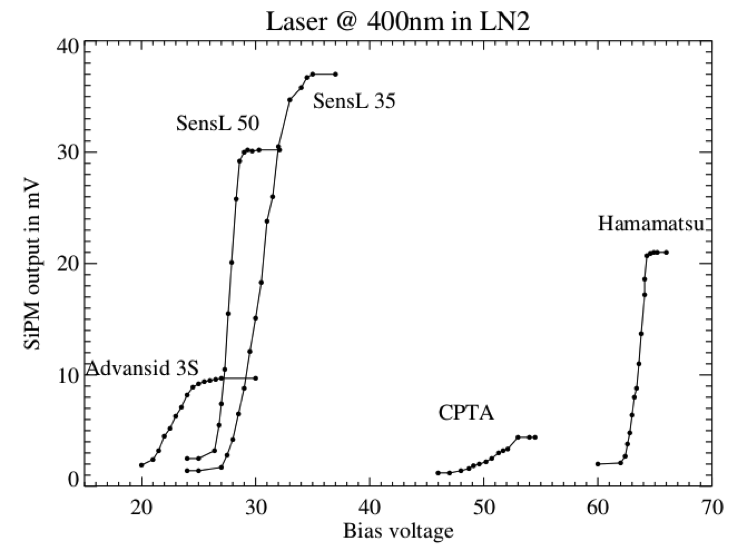
\includegraphics[width=.6\columnwidth]{sipm_laser.png}
\end{cdrfigure}

Based on these initial tests, the follow up tests focused on SenSL and
Hamamtsu models. This decision was partially driven by the high price
quotes received at the time from AdvanSiD and CPTA.

Shortly after initial tests, SenSL came up with a new model
(MicroFB-600-35-SMT followed by improved MicroFC-600-35-SMT) and most
of the tests have been done on the SenSL models. Hamamtsu’s MPPC
S12895- 0404-PB50 has been on the market for a long time and Indiana
group measured very high cross-talk and afterpulsing rates. Hamamtsu
came up with a new, improved model in 2015, S13360, that will be
tested in 2015 and compared with SenSL models.

\subsection{Requirements}

PD system requires high sensitivity photo-detectors to detect argon
scintillation light, despite its excellent scintillation yield due to
a very small surface area of the PDs.  The late scintillation light in
argon reprsents 2/3 of the total scintillation light, but it is spread
over 1100 - 1600~ns, making the individual late light signals very
small in average.

SiPM characteristics from the data sheets satisfy these requirements
in general. Thus, it is important to verify that similar performance
is observed at LAr temperatures in terms of high gain, sensitivity to
single photoelectrons, high PDE, linearity of the response, stability
of breakdown voltage, long-term stability, low afterpulsing and low
cross-talk. In addition, SiPMs must have low dark rate and mechanical
robustness as they undergo cryogenic cooling and cycling. Finally
devices must have low cost and we need to identify at least two
suitable choices to avoid sole source issues.

Institutions designing different PD prototypes (Indiana University,
Colorado State University and Louisiana State University) have
conducted a number of tests of PDs with SiPMs. Additional,
specifically targeted tests have been conducted at Louisiana State
University (LSU) and University of Hawaii (UH) in recent
months. Importance of selecting the best photo-sensors for the PD
motivates the need for parallel tests conducted at both LSU and
UH. Such approach will ensure important cross-checks and reduce
possible testing biases.

\subsection{Test Results}

In the last 18 months, we have built a test setup for SiPM evaluation,
that includes Belle experiment electronics to power and record signals
from SiPMs.  More recently, we have designed a new board similar to
SenSL testing board (to address noise problems and low amplification
of the Belle board critical at low light levels) that is currently
being used to conduct dark rate and single photoelectron study.
Fig~\ref{sipm_schem} shows the layout of the new testing board and
picture of the actual circuit as built.

\begin{cdrfigure}[The diagram on the left shows the schematics of the
    PCB board, while the picture on the right shows the PCB as
    built. This PCB can accommodate three SiPMs for
    testing.]{sipm_schem}{The diagram on the left shows the schematics
    of the PCB board, while the picture on the right shows the PCB as
    built. This PCB can accommodate three SiPMs for testing.}  
  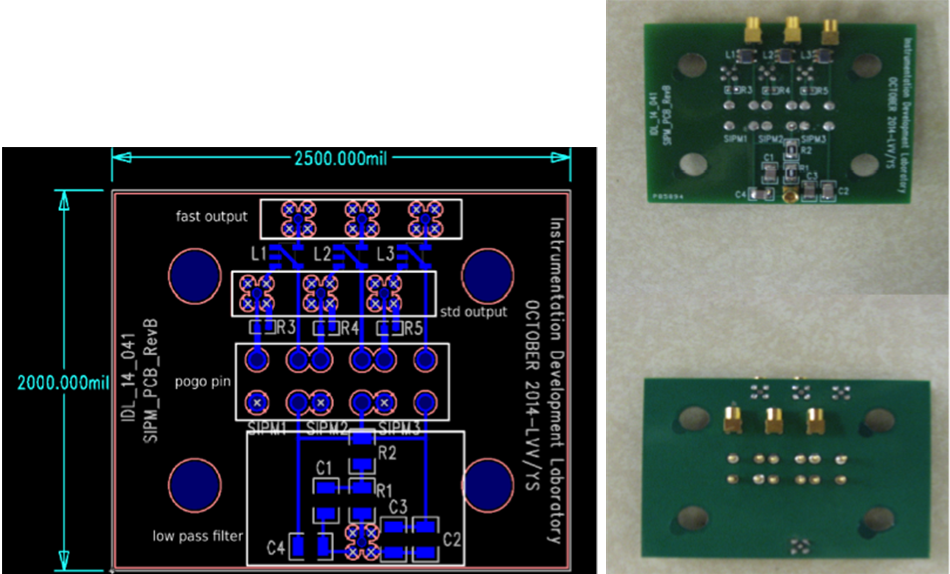
\includegraphics[width=.6\columnwidth]{pd_SiPM_schem.png}
\end{cdrfigure}

As previously mentioned, tests focused on Hamamatsu and SenSL produced
8 SiPMs. However, Indiana University group found out that Hamamatsu
SiPMs are placed in a dewar inside a copper plated dark box and cooled
with LN2. SiPMs are held in place on the PCB with acrylic holder as
shown in the Fig~\ref{sipm_mount}.

\begin{cdrfigure}[Picture on the left shows acrylic holder that
    secures SiPMs to the PCB while figure on the top right shows the
    entire assembly prior to lowering in the dewer. Orange cable
    delivers laser or LED light that shines on the SiPMs. Everything
    is secured to the wooden lid that closes the
    dewer.]{sipm_mount}{Picture on the left shows acrylic holder that
    secures SiPMs to the PCB while figure on the top right shows the
    entire assembly prior to lowering in the dewer. Orange cable
    delivers laser or LED light that shines on the SiPMs. Everything
    is secured to the wooden lid that closes the dewer.}   
  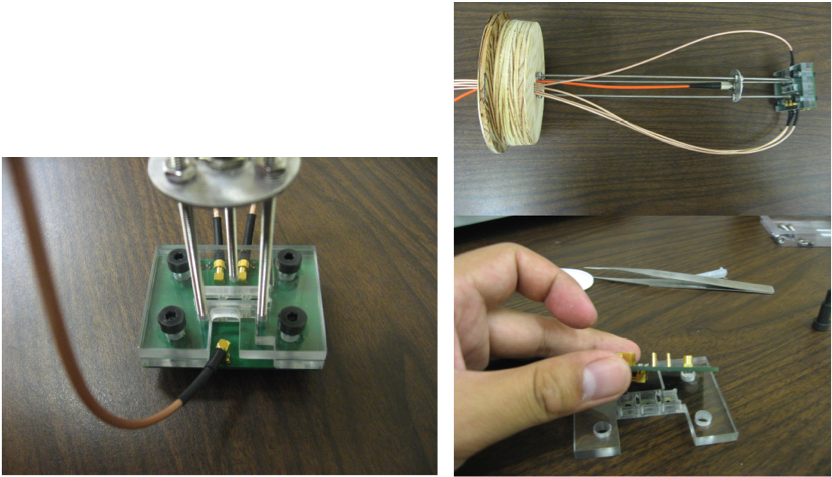
\includegraphics[width=.6\columnwidth]{sipm_mount.png}
\end{cdrfigure}

To address the issue of different contraction rates of materials in
LN2 that produced mechanical damage to some of the SiPMs, a PCB board
with spring loaded POGO pins is used (based on the previous design by
the Colorado State University group) to provide contact to SiPMs and
hold SiPMs in place with acrylic housing rather than solder joints. We
have also acquired special cryo rated, compact MMCX connectors, as the
solder joints of the signal and power wires have been breaking from
repeated usage.

The SiPM bias voltage is delivered via POGO pins and SiPM signal is
sent via POGO pins to the DAQ. The signal is amplified via two inline
low noise amplifiers and read out by oscilloscope. SiPMs are
illuminated by a 1~ns long laser pulses from the tunable wavelength
laser system. Laser light intensity is regulated with a Fine Laser
Intensity Controller (FLIC), a computer controlled system allowing us
to tune laser intensity through several orders of magnitude with
various stages, important for linearity measurements. Signal waveforms
from Waverunner LeCroy oscilloscope are recorded and analyzed
afterwards.

We have also noted that the SiPMs require lower bias voltage when
cooled in LN2, which requires determination of the optimal operating
voltage at LAr temperature as dark rates also increase with bias
voltage. Additional tests showed excellent gain at cryogenic
temperatures as can be seen from the tests conducted on the SenSL C
series SiPM MicroFC-600-35-SMT (previous M and B series also tested)
shown in Fig~\ref{sipm_gain}. along with clearly distinguished pulses
for 1, 2, 3 and 4 photelectron pulses.

\begin{cdrfigure}[SiPM SenSL C series gain tested in LN2 is shown on
    the right hand side. Excellent linearity over the entire
    overvoltage range observed. There is a significant change of gain
    with increasing bias voltage, effectively doubling between the
    minimum and maximum tested bias voltage. Clearly distinguished
    numbers of photoelectrons can be seen in the left hand
    figure.]{sipm_gain}{SiPM SenSL C series gain tested in LN2 is
    shown on the right hand side. Excellent linearity over the entire
    overvoltage range observed. There is a significant change of gain
    with increasing bias voltage, effectively doubling between the
    minimum and maximum tested bias voltage. Clearly distinguished
    numbers of photoelectrons can be seen in the left hand figure.}    
  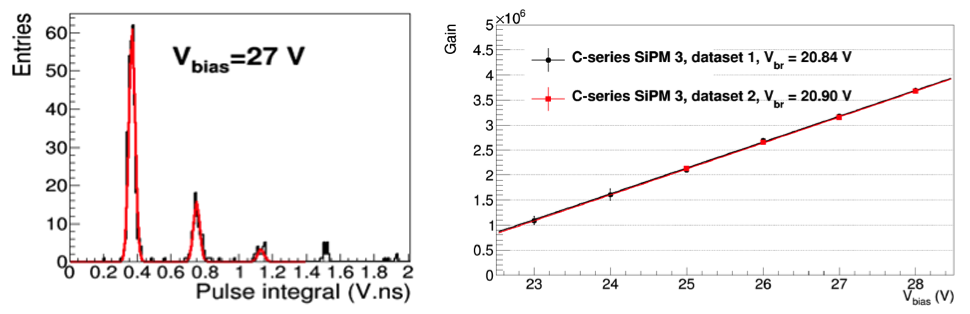
\includegraphics[width=1.0\columnwidth]{sipm_gains.png}
\end{cdrfigure}

The dark rate increases significantly with bias voltage, but the
overall rate is very small when SiPMs are cooled down to 80 K as can
be seen in Fig.~\ref{sipm_dark}.

\begin{cdrfigure}[SiPM SenSL C series dark rate with two different
    data runs in LN2. While dark rate increases for an order of
    magnitude, it is still less than 50 Hz even at the highest bias
    voltage setting.]{sipm_dark}{SiPM SenSL C series dark rate with
    two different data runs in LN2. While dark rate increases for an
    order of magnitude, it is still less than 50 Hz even at the
    highest bias voltage setting.}     
  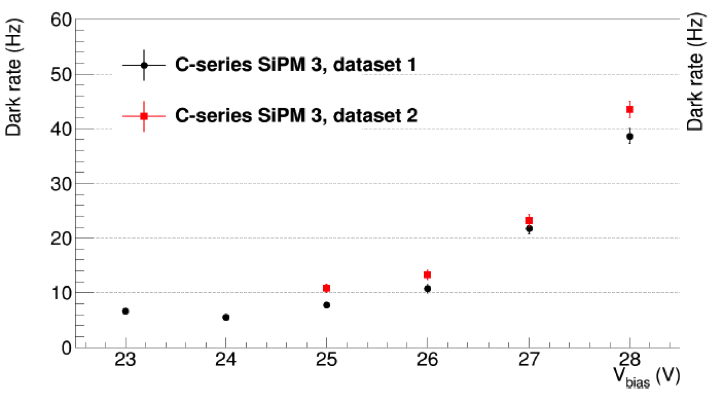
\includegraphics[width=0.6\columnwidth]{sipm_dark_rates.png}
\end{cdrfigure}

Afterpulsing is another important aspect of SiPM
performance. Afterpulsing increases noise and obstructs detection of
late argon scintillation light. Results of the afterpulsing
measurement performed on the SenSL C series, cooled down SiPM show
very small afterpulsing fraction below 1\% for most overvoltage
values, as can be seen in Fig.~\ref{sipm_after}.

\begin{cdrfigure}[SenSL C series SiPM afterpulsing fraction for 5
    different SiPMs, with system being completely cooled
    down.]{sipm_after}{SenSL C series SiPM afterpulsing fraction for 5
    different SiPMs, with system being completely cooled down.}      
  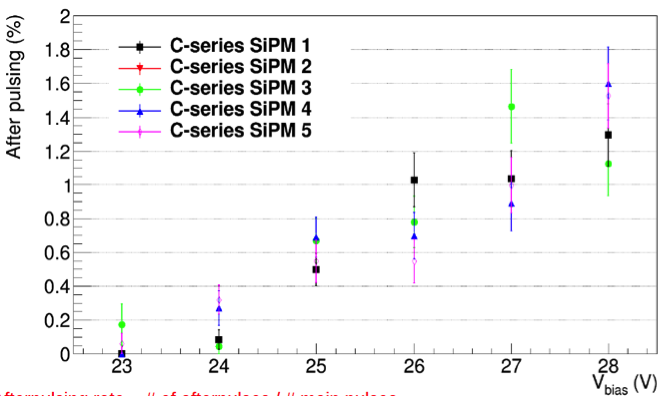
\includegraphics[width=0.6\columnwidth]{sipm_afterpulsing.png}
\end{cdrfigure}

SenSL C series SiPMs were also tested for cross-talk. Cross-talk gives
a measure of the light hitting one pixel, also produces signal in
adjacent pixels and effectively distorts the signal
strength. Fig.~\ref{sipm_crosstalk}. shows the test
results. Cross-talk is a strong function of overvoltage which will be
another criteria in choosing the operating overvoltage for the PD
system.

Although, not presented here, SenSL B series SiPM MicroFB-600-35-SMT
were also tested and satisfy our requirements, based on the tests
conducted so far. However, we have not performed yet a full set of
tests including mechanical integrity from thermal cycling and
cross-checks. 

\begin{cdrfigure}[SenSL C series SiPM cross-talk measurement based on
    two separate runs in LN2. Cross-talk is a strong function of
    overvoltage and is very consistent between the
    runs.]{sipm_crosstalk}{SenSL C series SiPM cross-talk measurement
    based on two separate runs in LN2. Cross-talk is a strong function
    of overvoltage and is very consistent between the runs.}       
  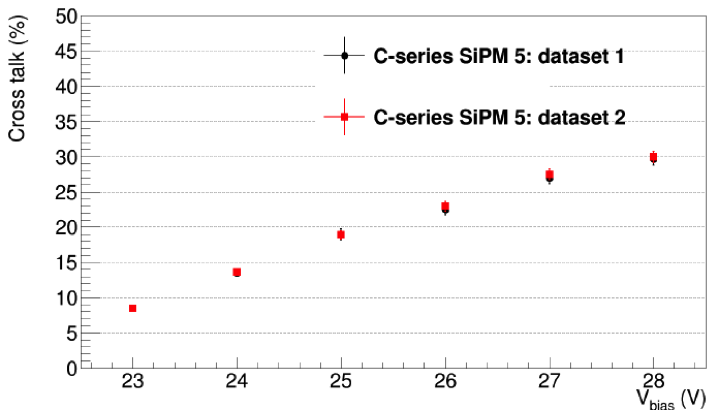
\includegraphics[width=0.6\columnwidth]{sipm_crosstalk.png}
\end{cdrfigure}

In parallel with performance test, mechanical cryogenic tests were
conducted where the number of cycles and time spent at LN2 temperature
has been logged. This important test has started recently, but will
involve testing a number of devices for extended period of time and
examining mechanical status under the microscope along with
performance tests. 

Future steps involve increasing the testing sample of C series SiPMs
and evaluating several alternatives to avoid the risk of sole source
vendor. 


\section{Mechanical Support}

Mechanically supporting the photon detector systems in the APA frames
presented several challenges, including the need to support three
different light collecting and wavelength shifting technologies in a
package utilizing the same mounting features in the APA frames, and
the effects of varying thermal contraction of various materials at 80
degrees Kelvin which complicated both light collector and SiPM
mounting.

The baseline design for mounting the PDs into the APA frames calls for
ten PD modules, approximately 2.2m long, mounted roughly equally
spaced along the full length of the APA frame (Figure~\ref{fig:5.5-1}).  The
PD modules are read out using individual twisted pair cable, one per
SiPM.  These cables (120 of them in the original baseline design) are
routed through the APA side tubes to a connector at the cold
electronics readout end of the APA.  Initially it was decided that it
would be too complicated to design the APA frames to allow PD module
installation following APA wire-wrapping, so the PD modules were
installed prior to this step in the installation process.  The
Wavelength shifting elements in the light collectors of the PD modules
are sensitive to heat, humidity and most critically to exposure to
ambient light, which places significant requirements on the
environment the APAs are assembled and stored in this way, but
initially it was decided this was the best option.

\begin{cdrfigure}[Full APA frame with ten photon detectors mounted
  inside the frame]{5.5-1}{Full APA frame with ten photon detectors mounted
  inside the frame}
   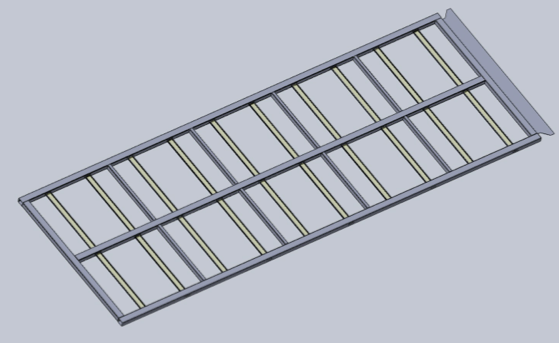
\includegraphics[width=.6\columnwidth]{fig5-5-1.png}
\end{cdrfigure}

A universal PD frame assembly was devised to hold all three PD design
variations under consideration.  Figure~\ref{fig:5.5-2} shows an example of a
short (400~mm long active area) version of this frame manufactured for
the 35t test, and Figure~\ref{fig:5.5-3} shows a mechanical assembly drawing of
the frame system for one of the candidate light collector choices.
The frame consists of two plastic (acetal) end caps mounted to the
inside of the APA frame, joined by 10~mm diameter stainless steel tubes
which run the full width of the APA frame, providing intermediate
support for the PD modules as needed.  The SiPM mount PCBs are
incorporated into one of the end blocks, along with the cable
connections for the twisted pair cables.  Due to the significant
variations in coefficient of thermal expansion between the stainless
steel frame and the plastic WLS elements, we expect a relative
difference in thermal contraction of ~1\% at LAr temperatures.  The
far endblock assembly provides balancing forces to the light collector
elements as required to ensure these elements remain in straight and
in good contact with the SiPMs.

\begin{cdrfigure}[Photograph of 40~cm long bar-based prototype mounted in test frame]{5.5-2}{Photograph of 40~cm long bar-based prototype mounted in test frame}
  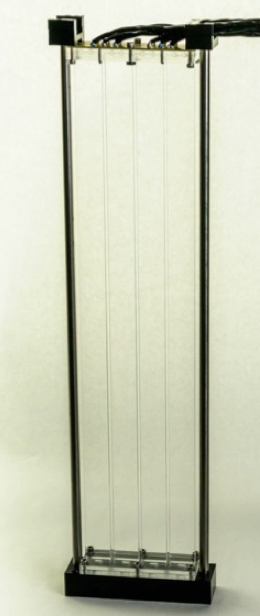
\includegraphics[width=.5\textwidth]{fig5-5-2.png}
\end{cdrfigure}


\begin{cdrfigure}[Mechanical assembly drawing of frame system]{5.5-3}{Mechanical assembly drawing of frame system}
  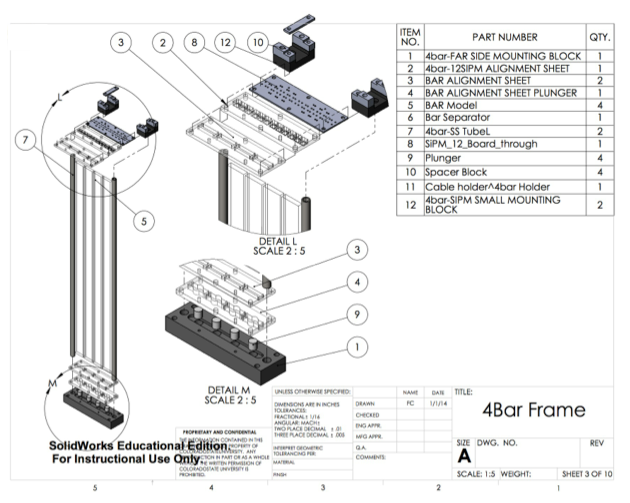
\includegraphics[width=.8\columnwidth]{fig5-5-3.png}
\end{cdrfigure}


Testing of the PD mount scheme in many test setups (at IU, CSU and
FNAL), as well as experience APA assembly, have led to a re-evaluation
of the PD mounting scheme.  The revised baseline has PD installation
occurring following APA wire wrapping, through slots left in the side
of the APA frame (Figure~\ref{fig:5.5-4}).  As shown in the figure, the
plan still calls for ten PDs per APA frame.  Five of the PDs will be
installed through each side of the APA frame, and the cables for each
of the PDs will be routed to the cold electronics end of the APA
inside the side tube the PD was inserted through.  Stainless steel
c-channels mounted into the APA frames prior to wire wrapping will
guide and support the PDs during and after installation.  The PD will
only be attached to the APA frame at one end, so the purely-plastic PD
module will be free to slide in the track to allow for the
differential contraction (Figure~\ref{fig:5.5-5}).  Tests of 2.2m prototype
assemblies of both fiber hybrid and the LSU-proposed monolithic
acrylic bar design in the CSU CDDF have demonstrated significant
promise.  This installation scheme

\begin{cdrfigure}[Blow up of APA fram showing PD insertion location]{5.5-4}{Blow up of APA fram showing PD insertion location}
  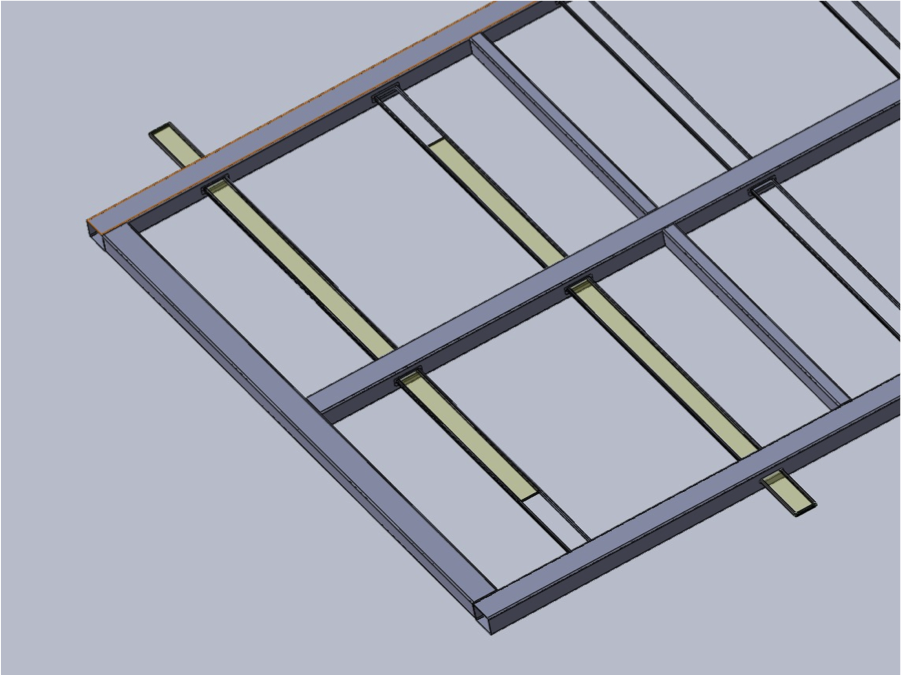
\includegraphics[width=.6\columnwidth]{fig5-5-4.png}
\end{cdrfigure}


\begin{cdrfigure}[Slot and rail showing mounting location of photon detector]{5.5-5}{Slot and rail showing mounting location of photon detector}
  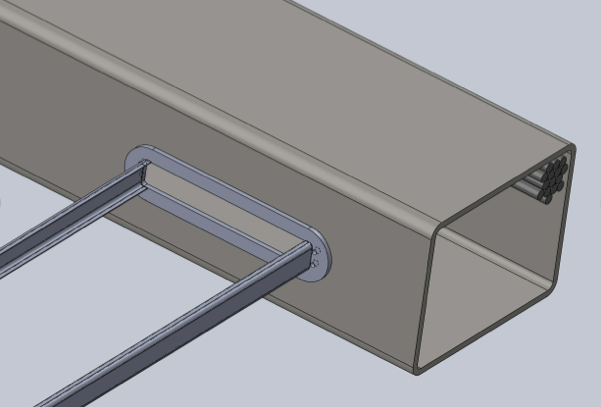
\includegraphics[width=.6\columnwidth]{fig5-5-5.png}
\end{cdrfigure}


Thermal contraction at cryogenic temperatures also complicates the
mounting of the SiPMs in the PD modules.  The baseline sensL SiPMs are
surface mount components, with 4 0.5~X~0.5mm pads for making
electrical contact.  Reliability and elevated dark count rate
problems, as well as physical delamination of the SiPM front face from
the silicone substrate, were observed early in cryogenic testing of
SiPMs, and suspicion fell on the mechanical contact between the
mounting PCB and the SiPM itself.

Three different methods of making these electrical contacts: Soldering
the SiPMs directly to the PCBs (fig 5.5-6a), using commercial
spring-loaded electrical contacts or “Pogo pins” (Figure~\ref{fig:5.5-6b}),\fixme{check ref} and
soldering short wires to the SiPM pads and thence to the PCB
(Figure~\ref{fig:5.5-6c}).\fixme{check ref}  Each of these methods provides assembly challenges,
and cryogenic testing has not suggested a clear choice so far.
Testing and development are still underway to resolve this issue.

\section{Photon System Readout Electronics}
\label{sec_elec}

\subsection{Reference Design} %Added by AH to avoid single subsec for Alternatives'

Scintillation light from LAr comes from the two different excited
states with lifetimes of about 6 ns and 1.6 $\mu$s.  Only a limited
amount of light is collected by this system, so the electronics must
be designed to collect the light from both excited states. A summary
of the general requirements for the system, including requirements
from a physics performance perspective, are given in
Table~\ref{tab:fee_req}.
%
\begin{cdrtable}[Physics requirements for the photon detector electronics]{ll}{fee_req}
{Physics requirements for the photon detector electronics}
 Performance Parameter       & Target   \\ \toprowrule
 Time Resolution                   & Better than 30 nS wrt event time zero ("t0")       \\ \colhline
 Charge Resolution               & 0.25\% photo-electron equivalent                      \\ \colhline
 Dynamic Range                   & $\sim$ x10 better than detector (1000:1)          \\ \colhline
 Linearity                               & Sufficient to resolve 1 photo-electron signals   \\ \colhline
 Multi-Hit Capability              & Sufficient to measure Triplet (late) Photons           \\ \colhline
 Dead Time                           & Live up to 2 drift times either side of beam spill           \\ \colhline
 Bias Control                        & 0.1 V resolution up to 30 V per channel   \\ \colhline
 Calibration                          & On-board Charge Injection   \\ \colhline
 Timing                                 & Events time-stamped using NO$\nu$A Timing syst.  \\
\end{cdrtable}


%
The plans for the electronics for the photon detection subsystem
include a baseline design with several options that remain R\&D
activities.  There alternative implementations of electronics are
described in Section~\ref{sec_alt}.
%These options are identified in the description that follows.  
%There are also some alternative implementations of electronics that remain under consideration.  These are described in Section~\ref{sec_alt}
%These are described in Section 6.4.

In the baseline plan, there are no front-end electronics in the cold
volume.  Instead, the un-amplified signals from the SiPMs are
transmitted to outside the cryostat on cables for processing and
digitization, as shown in Figure~\ref{fig:fig-e-1}.  There are
advantages and disadvantages to this approach.  The advantages are
that the infrastructure required for inside the cryostat is reduced
(power, data cables, precision clocks, data protocols, etc.);
reliability is improved (no single-point failures of multi-channel
devices inside the cryostat); serviceability and accessibility to the
front-end electronics are improved; and the need to develop cold
electronics, possibly a custom ASIC, is eliminated.  The disadvantages
are that the cable plant inside the detector is increased, which can
create mechanical challenges and installation difficulties; the flange
board (warm/cold interface) is more complex; there are generally more
connectors in the system; and signal-to-noise considerations are more
difficult.  Generally, the baseline design favors simplicity,
reliability and reduced R\&D time and costs, and also meets the
performance requirements of the electronics.
%
\fixme{No fig1 exists for: Block diagram of the photon detector signal processing system.  }
%
\begin{cdrfigure}[Block diagram of the photon detector signal processing system]{fig-e-1}{Block diagram of the photon detector signal processing system}
%\includegraphics[angle=0,width=10cm,height=7cm]{fig1}
\end{cdrfigure}

In the 35-ton prototype, each SiPM signal was transmitted on an
individual shielded twisted-pair cable fitted with individual
LEMO-style connectors.  The bias voltage was coupled onto the signal
cable, using AC-coupling on the receiving end to measure the SiPM
signal.  The use of high-quality cable with point-to-point connections
between an individual SiPM inside the cryostat and the front-end
electronics residing outside the cryostat, combined with good
differential signal processing on the receiving end, enabled the
demonstration of the principle that single photo-electron signals
could be measured accurately without the need for cold electronics.
In order to address the problems with the cable plant as identified
above, the following ideas are being pursued:
\begin{itemize}
\item Ganging together of several SiPM outputs from a given PD
  detector into one output cable.  This increases the detector
  capacitance, affects the pulse shape, and could spoil the timing
  resolution of the measurement.  Also, the SiPMs may have to be
  preselected, since there will be only one bias voltage for three
  devices, and it may be important to match the over-voltage
  characteristics.  Studies are in progress to find a compromise
  between data precision and cabling issues. One approach is to add a
  cold pre-amplifier if the ganging together of several SiPMs result
  in performance that is too degraded to meet specifications.  The
  infrastructure requirements (cables, connectors, power, cold
  performance, reliability, mechanical mounting, etc.) would have to
  be considered.

\item Use of multi-conductor, individually shielded pair cable.  A
  candidate cable containing four individually-shielded twisted pairs
  has been identified and tests are in progress.  The cable is in
  Teflon jacket, which should be acceptable for use in LAr.

\item Use of mass-terminated connectors.  Several candidate connectors
  for use with the cable described above are being pursued.
\end{itemize}

The baseline plan assumes that three SiPM signals can be ganged
together into one readout channel.  By using the multi-conductor cable
with four twisted pairs, this results in one cable per PD consisting
of 12 SiPMs.  The diameter of this cable is ~xxx mm, which reduces the
cable plant by $\sim$ x10 compared to that used in the 35 ton
detector.  The cost of the connectors also decreases by $\sim$ x10.
Lastly, the ease in making connections at the flange board will be
improved by the use of a mass-terminated connector.

In the baseline plan, the front-end electronics resides outside of the
cryostat in instrumentation racks.  We have designed and built a
custom module for receiving SiPM signals, and performing signal
processing in the front-end as preprocessing for trigger and DAQ.  The
module is called the SiPM Signal Processor (SSP).  An SSP consists of
12 readout channels packaged in a self-contained 1U module.  Each
channel contains a fully-differential voltage amplifier and a 14-bit,
150 MSPS analog-to-digital converter (ADC) that digitizes the
waveforms received from the SiPMs.  The front-end amplifier is
configured as fully-differential with high common-mode rejection, and
receives the SiPM signals into a termination resistor that matches the
characteristic impedance of the signal cable.  Currently there is no
shaping of the signal, since the SiPM response is slow enough relative
to the speed of the digitization to obtain several digitized samples
of the leading edge of the pulse for the determination of signal
timing.

The digitized data is stored in pipelines in the SSP, for up to $\sim$
13 $\mu$s.  The processing is pipelined, and performed by a Xilinx
Artix-7 Field-Programmable Gate Array (FPGA).  The FPGA implements an
independent Data Processor (DP) for each channel.  The processing
incorporates a leading edge discriminator for detecting events and a
constant fraction discriminator (CFD) for sub clock timing resolution.
Because the FPGA is programmable and accessible, it is possible to
explore different data processing algorithms and techniques, and even
customize the readout for a given type of event (supernova for
example.)  A picture of the module is shown in Figure~\ref{fig:fig-e-2}.
A block diagram of the system is shown in Figure~\ref{fig:fig-e-3}.

%Figure xx3.  Picture of the SSP module.
\begin{cdrfigure}[Picture of the SSP module]{fig-e-2}{Picture of the SSP module}
%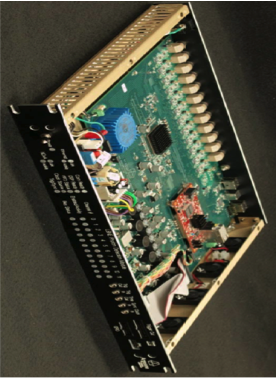
\includegraphics[angle=90,width=10cm,height=5cm]{fig-e-2.png}
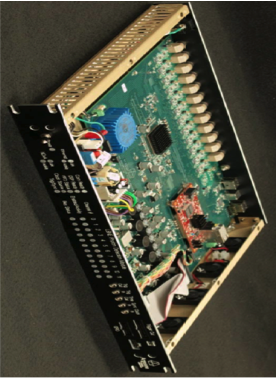
\includegraphics[angle=90,width=.8\textwidth]{fig-e-2.png}
\end{cdrfigure}

%Figure xx2.  Block diagram of the SSP.
\begin{cdrfigure}[Block diagram the SSP module]{fig-e-3}{Block diagram the SSP module}
%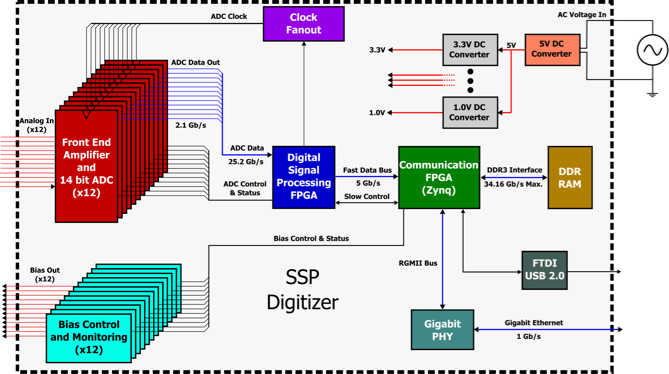
\includegraphics[angle=0,width=12cm,height=7cm]{fig-e-3.png}
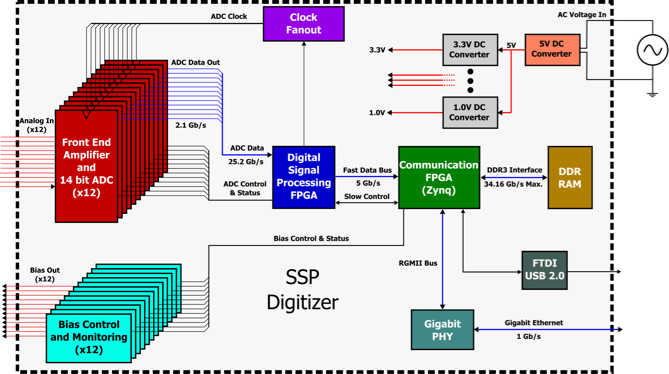
\includegraphics[angle=0,width=.95\textwidth]{fig-e-3.png}
\end{cdrfigure}

In the simplest mode of operation, the module can perform waveform
capture, using either an internal trigger or an external trigger.  Up
to 2046 waveform samples may be read out for each event.  When
waveform readouts overlap the device can be configured to offset,
truncate or completely suppress the overlapping waveform.  Pile-up
events can also be suppressed.

As an alternative to reading full waveforms, the DP can be configured
to perform a wide variety of data processing algorithms, including
several techniques for measuring amplitude, and also timing of the
event with respect to a reference clock.  All timing and amplitude
values are reported in a compact event record.  Each data processing
channel stores up to 340 event records when not storing waveforms.

Generally, the SSP performs pipelined processing.  The module has been
designed to support several different triggering schemes, including
self-triggered, use of an external trigger, or use an external gate to
readout all events within a time-window.  In order for the events
measured in the photon detector to be matched up with the
corresponding events in the TPC, the front-end electronics attaches a
timestamp to the data as it is acquired.  The timestamp is unique, and
has a correspondence with the timestamps in the TPC electronics
processing.  The timestamp in the SSP is applied to the event data as
it is digitized, and becomes part of the data as the processing
proceeds.  In the case where zero-suppression and data sparsification
are used, the timestamp on accepted data remains intact.  To achieve
this, the TPC and PD electronics must be synchronized, including
timestamp counter resets, and a known and stable calibration between
the corresponding timing resolution of the ADC conversion in the two
systems.  The electronics has been designed to support a full
interface to the NO$\nu$A timing system, which is the baseline timing
system for the experimental prototypes.

A Xilinx Zynq FPGA, onboard the MicroZed system-on-module, handles the
slow control and event data transfer.  The SSP has two parallel
communication interfaces; USB 2.0 and 10/100/1000 Ethernet.  The 1
Gb/s Ethernet supports full TCP/IP protocol.  The module includes a
separate 12-bit high-voltage DAC for each channel to provide up to 30
V of bias to each SiPM.  The module also feature charge injection for
performing diagnostics and linearity monitoring, and also voltage
monitoring.

In tests to date, the SSP is capable of measuring single
photo-electron signals coming from the SiPMs over a cable length of 30
meters when the SiPMs are operated at LAr temperatures.  The timing
resolution of the signals has been measured to be better than 3 ns.
The full-differential signal processing in the front-end circuitry is
important in achieving this result.
 
The SSP is self-contained in that it receives 60 Hz, 120V power, and
has internal linear and DC/DC power supplies for generating the DC
voltages needed for the instrumentation, as well as the bias voltage
for the SiPMs.  The SSP is packaged in a 1U, rack-mountable
package. For the 35-ton prototype, the racks are located near the
ports on the top of the cryostat.

\subsection{Alternatives}
\label{sec_alt}

In the baseline design of the PD electronics, the approach was taken
to have no electronics inside of the cold volume.  This results in a
large number of cables and connectors.  Other experiments using liquid
argon have successfully implemented cold TPC electronics, thereby
significantly reducing the cable plant that must come through the
cryostat.  

This approach has challenges in power distribution, heat
dissipation, and the performance of front-end electronics in LAr. To
address serviceability, the cold electronics might be realized in a
modular way and situated just below the flange in the cryostat so that
it can be accessed in the event that repair is needed.  To this end
the zero-suppression will be important to avoid high data rates
depending on the number of readout channels needed. A way to realize
the cold zero-suppression would be to implement a cold FPGA (or an
ASIC, yet to be developed).  So far the cold FPGAs have had mixed
results in tests. 

An alternative approach would be to perform an ``analog
zero suppression'' with a constant-fraction discriminator and then gate
the signal and digitize warm, in which case the complication with
encoding the particular channel has to be addressed.  The significant
challenges in this technique include power dissipation, the increased
possibility of contamination of the LAr, and extended infrastructure
requirements that must reside in the cold volume.  The virtue is that
this can significantly reduce the number of signal penetrations into
the cold volume.

The electronics for the photon detector of LBNE uses fast (direct)
digitization of the SiPM pulses. Another option for the front-end
electronics is to use pulse shaping. Instead of digitizing the full
bandwidth of the SiPM signal, the pulse is shaped using analog
filtering techniques, generally producing a pulse with a prescribed
shape with a peak that is proportional to the total amount of charge.
By measuring the peak, both amplitude and pulse timing can be
obtained.  Since the pulse response follows a known transfer function,
the pulse peak can be obtained using slower synchronous sampling, or
using asynchronous sampling through the use of peak detection and
constant fraction discrimination.  

In either case, the data can be
processed by an FPGA using algorithms optimized for the application.
In particular, assuming that a sufficient number of samples are
obtained of the shaped pulse, a chi-square comparison of the shape to
the ideal pulse can be used to determine pulse corruption, or event
identification.  As with direct digitization, the digitization clock
and timestamp can be synchronized using an external clock source. The
data can be read out in a similar manner, using USB 2.0 or 10/100/1000
Ethernet.  The virtue of this approach is that a slower ADC can be
used, reducing power consumption, and also reducing data load and the
speed of readout links.  The technique does trade bandwidth for
shaping, making timing and pile-up issues more important.  This can
result in the interpretation of the pulse shape becoming more complex
than direct digitization.  Generally, the pulse shaping circuitry is
also less expensive than the direct digitization technique, assuming
similar performance requirements.

Another option for the photon system readout would include the use 
of an Application Specific Integrated circuit (ASIC) as a way to
reduce cost.  The large channel count in a real detector system is
such that the production cost of the system could be greatly reduced.
Often, the cost of development of an ASIC from scratch is quite high,
of order $\sim$400K, and can take $\sim$1 to 2 years for development, so cost
and schedule must be weighed carefully.  However, other benefits from
the ASIC approach include reduced space requirements for circuitry on
the front-end, lower power dissipation, and specialized functionality
in the front-end chip.  

There exist several ASICs that have been
designed over the last few years especially for SiPM readout.  One
could potentially explore the functionality and performance of these
designs, and evaluate their suitability for LBNE.  This option might
be used either for warm or cold electronics.  Direct digitization has
the virtue of being straight-forward from a circuit design
perspective.  By taking advantage of modern high-bandwidth OP amps,
high-speed, high-rate ADCs, and powerful FPGAs with high-speed serial
links, it is possible to obtain 14-bit dynamic range digitization with
$\sim$1 ns timing resolution.  By reading all of the samples into an
FPGA having a deep buffer, digital signal processing techniques can be
employed using the programmable logic, offering powerful analysis
algorithms that can be developed in time.  The technique generally has
higher power consumption and tends to be more expensive than simpler
instrumentation techniques.

\section{Photon Detector Calibration}
\label{sec_pd_calib}

The photon detector calibration is a part of a larger calibration plan
that covers all aspects of an LAr detector calibration, and includes
methods to convert collected charge to initial particle?s energy, as
well as calibration techniques to convert collected scintillation
light into estimate of particle's interaction time, energy, and a
track/vertex location for each event.  

As already described, the
baseline for the scintillation photon detectors assumes employment of
acrylic light collection paddles to reduce the required costly
photo-cathode area. Several photon detector designs are presently
being developed and are being tested in small dewars. Since each of
these new elements has not yet been tested in a large-scale TPC, the
35-ton LArTPC prototype is being constructed to provide essential
design validation. 

The current FD designs are anticipated to have
sufficient sensitivity to provide event timing information for
atmospheric neutrino and proton decay channels. However, it will not
provide high efficiency down to the 5-MeV neutrino energy level
desired by the supernova program. This would have the impact that the
event reconstruction energy resolution would be 20\% rather than 5\%
achievable with the event time determination from a photon detector
able to operate efficiently at a sufficiently low energy
threshold. The improvement in physics will be studied in the near
future but a substantial effort in development of improved detection
techniques is desired. 

In the absence of precise physics requirements
for the photon detector system and in order to support R\&D activities
on the photon detector development it was decided that the photon
detector should provide a time stamp to determine the time of
occurrence of an event (so called ``time zero'') with an accuracy much
better than 1 s \fixme{fix}.  

Items relevant to the photon detector calibration
are the fast and slow components of the light, photon propagation
including scattering and reflections, impact of N2, E-field strength,
as well as the energy range of interest. A calibration system that
addresses the issues listed above has to be both comprehensive and
cost-effective, and has to be tied to the overall calibration system
that includes both charge and scintillation light calibration
techniques. Such a system will be designed in the future.  

To support
the PD R\&D phase we designed a light-flasher based calibration system
that will serve to monitor the relative performance and time
resolution of the system. In particular, for anticipated 35-ton
performance tests we need to evaluate relative efficiencies of
multiple light collection techniques in order to be able to
down-select an optimal light readout technology. The system that meets
these requirements will consist of a set of LEDs as light sources or a
laser with a VUV wave-length, coupled to quartz fibers, thus
transmitting light from outside the detector volume to desired
locations at the CPA within a TPC. Therefore we will equip the 35-ton
detector with LEDs located and fired externally, with fibers running
into the cryostat, to diffusers that will emit light from the CPA to
the APA. 

For the 35-ton cryostat at the surface at Fermilab it will be
complementary to cosmic ray muon tracks as means of calibration. In
terms of light sources the measurements should be performed with an UV
(245-375nm) light source. The UV light mimics physics starting from
the wavelength shifter conversion, light guide propagation,
photo-sensor detection and FEE readout.  The external light-flasher
calibration system is designed under following assumptions:
\begin{itemize}
\item simple to implement (no active components within PD/APA, such as
  LEDs or fibers mounted within APA).
\item less-intrusive (less material within detector in terms of
  fibers, then equipping each PD frame with individual fiber).?\item
  provide a benchmark light-based reconstruction with the use of
  localized light sources distributed throughout the detector volume.
\item has a potential to be adapted for deployment in a large Far
  Detector in the future
\end{itemize}

We describe the system in Figure~\ref{fig:fig-c-1}. . The system
consists of a 1U rack mount Photon Detector Calibration Module (PDCM)
sitting outside the liquid argon cryostat. The module generates light
pulses that propagate through a quartz fiber-optic cable to diffusers
at cathode-plane (CPA) to distribute the light uniformly across the
photon detectors mounted within anode plane (APA).  There are 5
diffusers on the CPA plane: one in the center and four diffusers close
to the CPA corners, as shown in Figure~\ref{fig:fig-c-2}. 

%
\begin{cdrfigure}[Concept of the UV-light calibration system]{fig-c-1}{Concept of the UV-light calibration system for the photon
  detector in liquid argon}
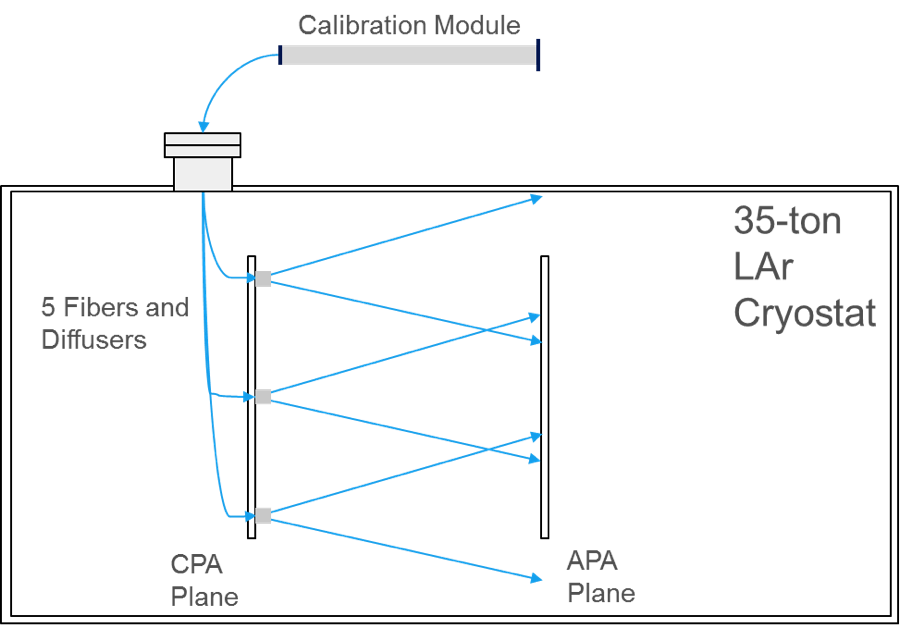
\includegraphics[angle=0,width=10cm,height=7cm]{fig-c-1.png}
\end{cdrfigure}


\begin{cdrfigure}[Diagrams of diffusers, their locations and UV light transport]{fig-c-2}{The diffuse light is emitted from diffusers (top left figure)
  mounted at five CPA locations, indicated by arrows (right figure).
  The UV light from the PDCM to diffusers is transported through
  quartz fiber (lower left figure).}
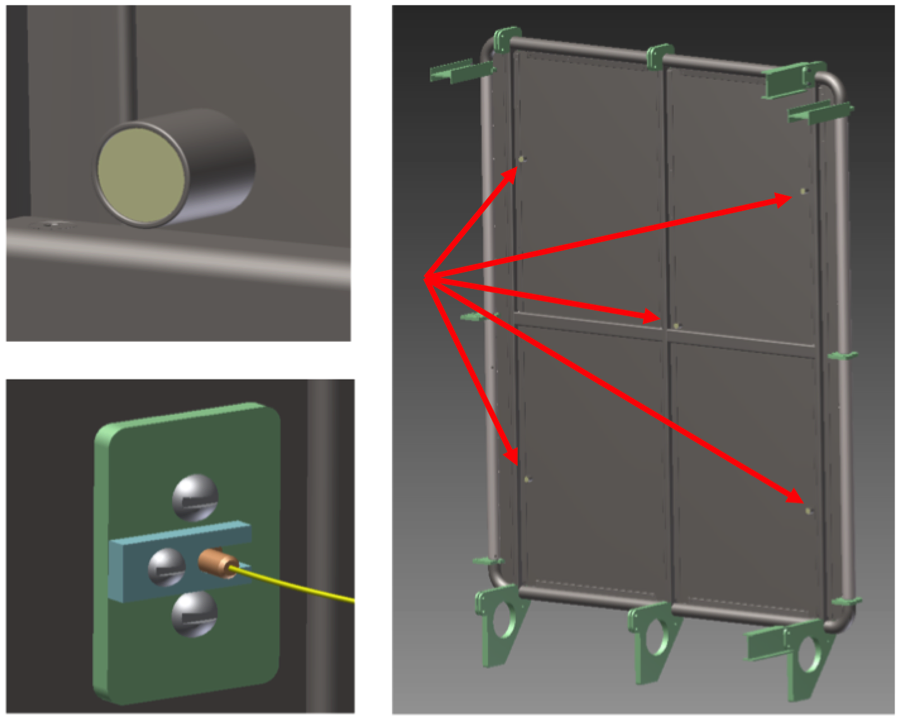
\includegraphics[angle=0,width=10cm,height=7cm]{fig-c-2.png}
\end{cdrfigure}


The PDCM module layout is shown in Figure~\ref{fig:fig-c-3}. The ANL
photon calibration module is based on a re-purposed SSP unit.  An SSP
board will be repackaged into a deeper rack mount chassis that will
accommodate a new internal LED Pulser Module (LPM) and an additional
bulk power supply. The LPM utilizes five digital outputs to control
the LPM pulse and its duration (arrows in black).  These LVDS outputs
are derived from the charge injection control logic within the SSP?s
FPGA.  The even channel SiPM bias DACs are repurposed to control the
LPM pulse amplitude (arrows in red).  The adjacent odd channels are
used to readout a photodiode which is used for pulse-by-pulse
monitoring of the LED light output.  The output of the monitoring
diode is used to normalize the response of the SiPMs in the detector
to the calibration pulse

\begin{cdrfigure}[Photon detector calibration module (PDCM) layout]{fig-c-3}{Photon detector calibration module (PDCM) layout}
%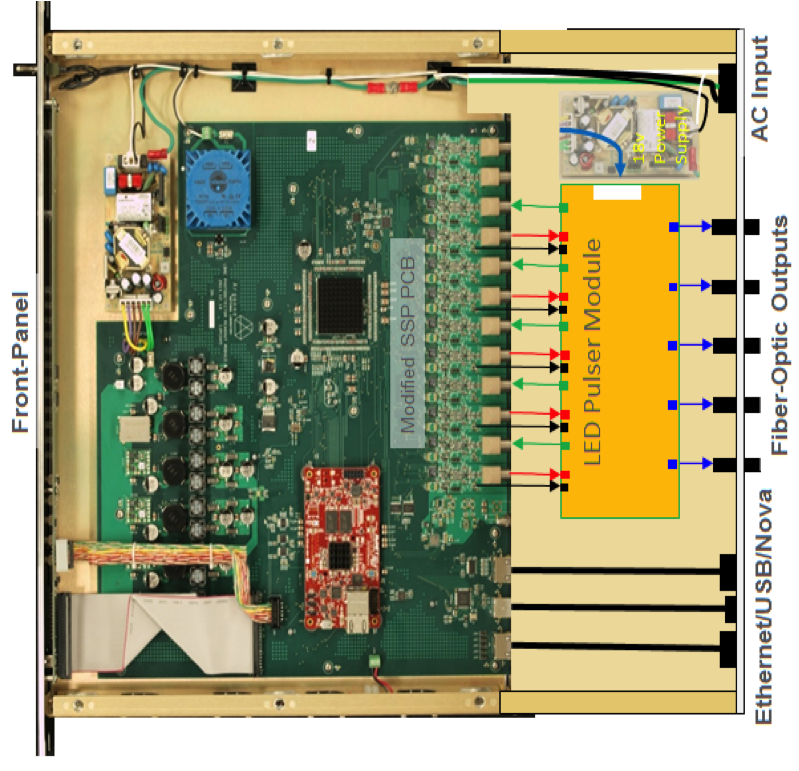
\includegraphics[angle=0,width=10cm,height=7cm]{fig-c-3.png}
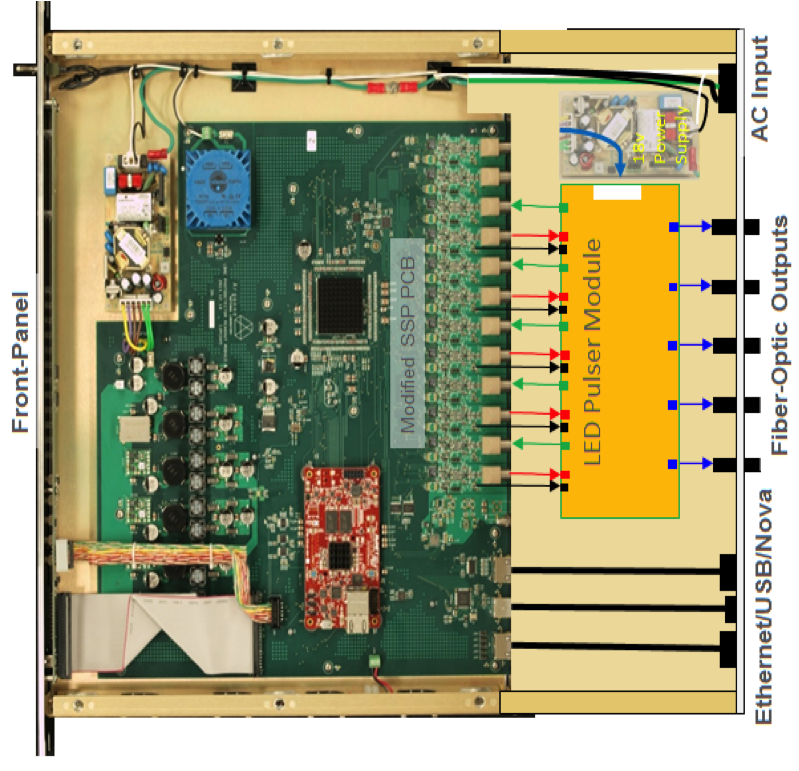
\includegraphics[angle=0,width=.8\textwidth]{fig-c-3.png}
\end{cdrfigure}


For the 280 nm light we have performed a simulation of the designed
diffuse light calibration system using TracePro, a generalized 3-D
light ray-tracing program with the ability to include bulk optical
properties such as absorption, fluorescence, birefringence in addition
to surface properties such as scattering and
reflection. Figure~\ref{fig:fig-c-4} shows simulated light distributions
of at the 35-ton APA for the cases of the VUV light emitted by either
the central diffuser only (left figure), or by outer four diffusers
simultaneously (right figure). A full Geant4 based simulation of the
detector will be used in the future. Using the preliminary data with
the 35-ton style light guides (indicating 0.5\% efficiency for number
of photo-electrons per incident 128 nm LAr scintillation photon 50 cm
from the light guide), we estimate for 280 nm light to observe ~15
photo-electrons per single SiPM channel when the light is emitted from
the single central diffuser in 13 ns long pulses. Similarly, we expect
about ~100 photo-electrons observed by a single SiPM channel when 280
nm light is emitted in 100 ns long pulses from the four outer
diffusers at once.

%
\begin{cdrfigure}[Simulated light distributions of the 35-ton APA, two cases]{fig-c-4}{Simulated light distributions of the 35-ton APA for the cases of the VUV light emitted by either the central diffuser only
  (left), or by outer four diffusers simultaneously (right).}
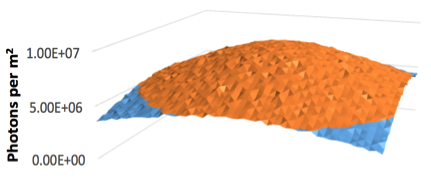
\includegraphics[angle=0,width=6.5cm,height=3.5cm]{fig-c-4-L.png}
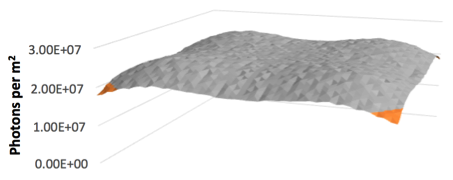
\includegraphics[angle=0,width=6.5cm,height=3.5cm]{fig-c-4-R.png}
\end{cdrfigure}


In the LBNE prototypes (i.e. in 35-ton) and in Future Far Detector it
will be important to check if photon-detector components are
functioning properly at various stages of the detector
operation. Periodic light source deployments will monitor the systems
stability as a function of time. A change in relative difference of UV
light responses will indicate towards potential wave-length shifter
instability, changes in SiPM gain and collection efficiencies. Much of
the same monitoring is expected to be doable with cosmic rays in the
35-ton (at surface), with periodic LED/laser calibration runs
complemented with cosmic-ray data tracked with an external
hodoscope. With the 35-ton detector one could use a well-defined muon
trajectory defined by the hodoscope geometry and monitor the number of
PEs per MeV of deposited charge. The number of PEs per PD channel from
the well-defined muon track could be used as a calibration
constant. However, for the deep underground LBNE the cosmic ray flux
may inadequate for timely monitoring of the photon detectors.  With
the 35-ton detector we have planned two sets of calibration runs:
\begin{enumerate}
\item Calibration runs with four outer diffusers run simultaneously,
  in order to\\ -measure response of PD channels in multi-PE range and
  get integrated number of event samples for each channel (for maximum
  light output)\\ -test of the dynamic range from 1PE to maximum
  number of PEs. \\ -repeat runs periodically to trace any changes in
  channel response.
       
\item Runs with central diffuser only, in order to\\ -perform initial
  calibration runs that will reveal malfunctioning channels, if
  any.\\ -timing measurements with the 10-50 ns pulses, verify time
  resolution of the PD system.
\end{enumerate}

The controlled source of light described here will be used to perform
a relative ?t0? calibration, where the ?t0? could be absolutely
calibrated with the use of the cosmic ray triggers available with
35-ton detector. Effects that contribute to a finite time resolution
and relative time offset of PD channels include scintillation time
constants, photon conversion with wave-length shifter, photon
propagation through PD paddle, SiPM jitter, and FEE resolution. Most
these effects are constant and can be individually measured on the
bench, so the LED flasher system will monitor overall stability of the
photon detector.  To go beyond the current R\&D phase one needs
detailed MC simulations of light production, propagation, and
detection to perform comparisons of reconstruction performance against
prototype data in terms of calorimetric energy and position
reconstructions for measured event tracks. Future light collection
systems will aim to maximize the active area of the light guide bars,
to achieve a high photon detection efficiency with an optimized timing
and granularity required for improved position resolution. As in the
case with the TPC charge calibration we will need to evaluate what may
be achieved with expected cosmic ray muons and Michels, $\pi^0$, and
natural radioactivity events (such as $^{39}$Ar with end-point energy
of abut 500 keV).

\section{Installation}

Installation of the photon detectors is one of the most significant
factors driving the mechanical design.  As discussed above, out
initial thought was to install the PDs and run the SiPM twisted pair
cable down the frame side tube prior to wire-wrapping the APA.
Following our experience with the environmental controls (primarily UV
filtered light) required by the PDs, as well as the difficulties in
dealing with the PD readout cable ends during wire-wrapping, it was
decided to change the baseline to include inserting the PDs following
wire wrapping.  In addition to relaxing the physical constraints on
the wire wrapping, this also relaxes a schedule connection between the
APA and PD fabrication.  It is not necessary to install the PDs into
the APA frames until shortly prior to installation of the APAs into
the cryostat.

As noted above, and shown in Figure~\ref{fig:5.5-4}, a total of 10 PDs are
installed into each APA frame, with 5 coming in from each side.  The
installation will occur with the fully-assembled APA frame lying flat
on an insertion station table.  Prior to installation, the PD cable
bundle will be inserted into the APA side tubes.  The cable bundle
will be pre-assembled prior to installation such that the end of each
cable will terminate at the correct slot for the PD to be connected.
Our baseline cable design has also been modified to a single cable
with 4 individual twisted pairs in a single jacket, so each APA side
tube will only require 15 cables (3 per PD, 30 per APA).  These cables
extend approximately 30cm past the end of the APA tubes at the cold
electronics end of the APA, and following installation of the APA into
the cryostat are connected to long-haul cables for the run to the
readout electronics (see Figure~\ref{fig:5.8-1}-- cable diagram).  Needs to be
made)

Following this step, 5 PDs will be inserted into the APA through one
side frame, with connections being made between the twisted pair
cables and the SiPM PCB just as the readout end of the detector enters
the tube (See Figure~\ref{fig:5.8-2}).  The PD is then inserted the last 10cm into
the frame, and affixed to the inner surface of the APA tube (See
Figure~\ref{fig:5.8-3}).  The process is then completed for the 5 PDs to be
inserted from the opposite side.

Following insertion of the PDs, the environmental controls required
for the PD WLS materials (UV filtering, temperature and humidity
control) will need to be observed for the entire APA.






